\documentclass[aspectratio=169,10pt]{beamer}
\usetheme{Madrid}
\setbeamertemplate{navigation symbols}{}
\setbeamertemplate{footline}[frame number]
\usepackage{amsmath,booktabs,graphicx}
\graphicspath{{../assets/}}
\newcommand{\src}[1]{\vfill{\tiny\color{gray}Source: #1}}
\title{LoRA and O-LoRA: Parameter-Efficient Fine-Tuning of Large Models}
\author{Thien-Lac Quach \and Minh-Quan Pham Nguyen \and Tinh Nguyen Van}
\institute{CS420 Seminar}\date{12 November 2026}
\begin{document}
\begin{frame}\titlepage\end{frame}
% Quan: 1 minute
\begin{frame}{Guiding question and scope}
\large How much does LoRA reduce trainable parameters, and what evidence is needed to assess quality and resource use?
\medskip\begin{itemize}
\item Derive counts for a $1024\times1024$ weight matrix.
\item Review LoRA and O-LoRA in their different task settings.
\item Examine the reported DistilRoBERTa evaluation on four-class AG News.
\end{itemize}\src{Report, Introduction and Abstract.}\end{frame}
% Quan: 1 minute
\begin{frame}{Ways to adapt a pretrained model}
\centering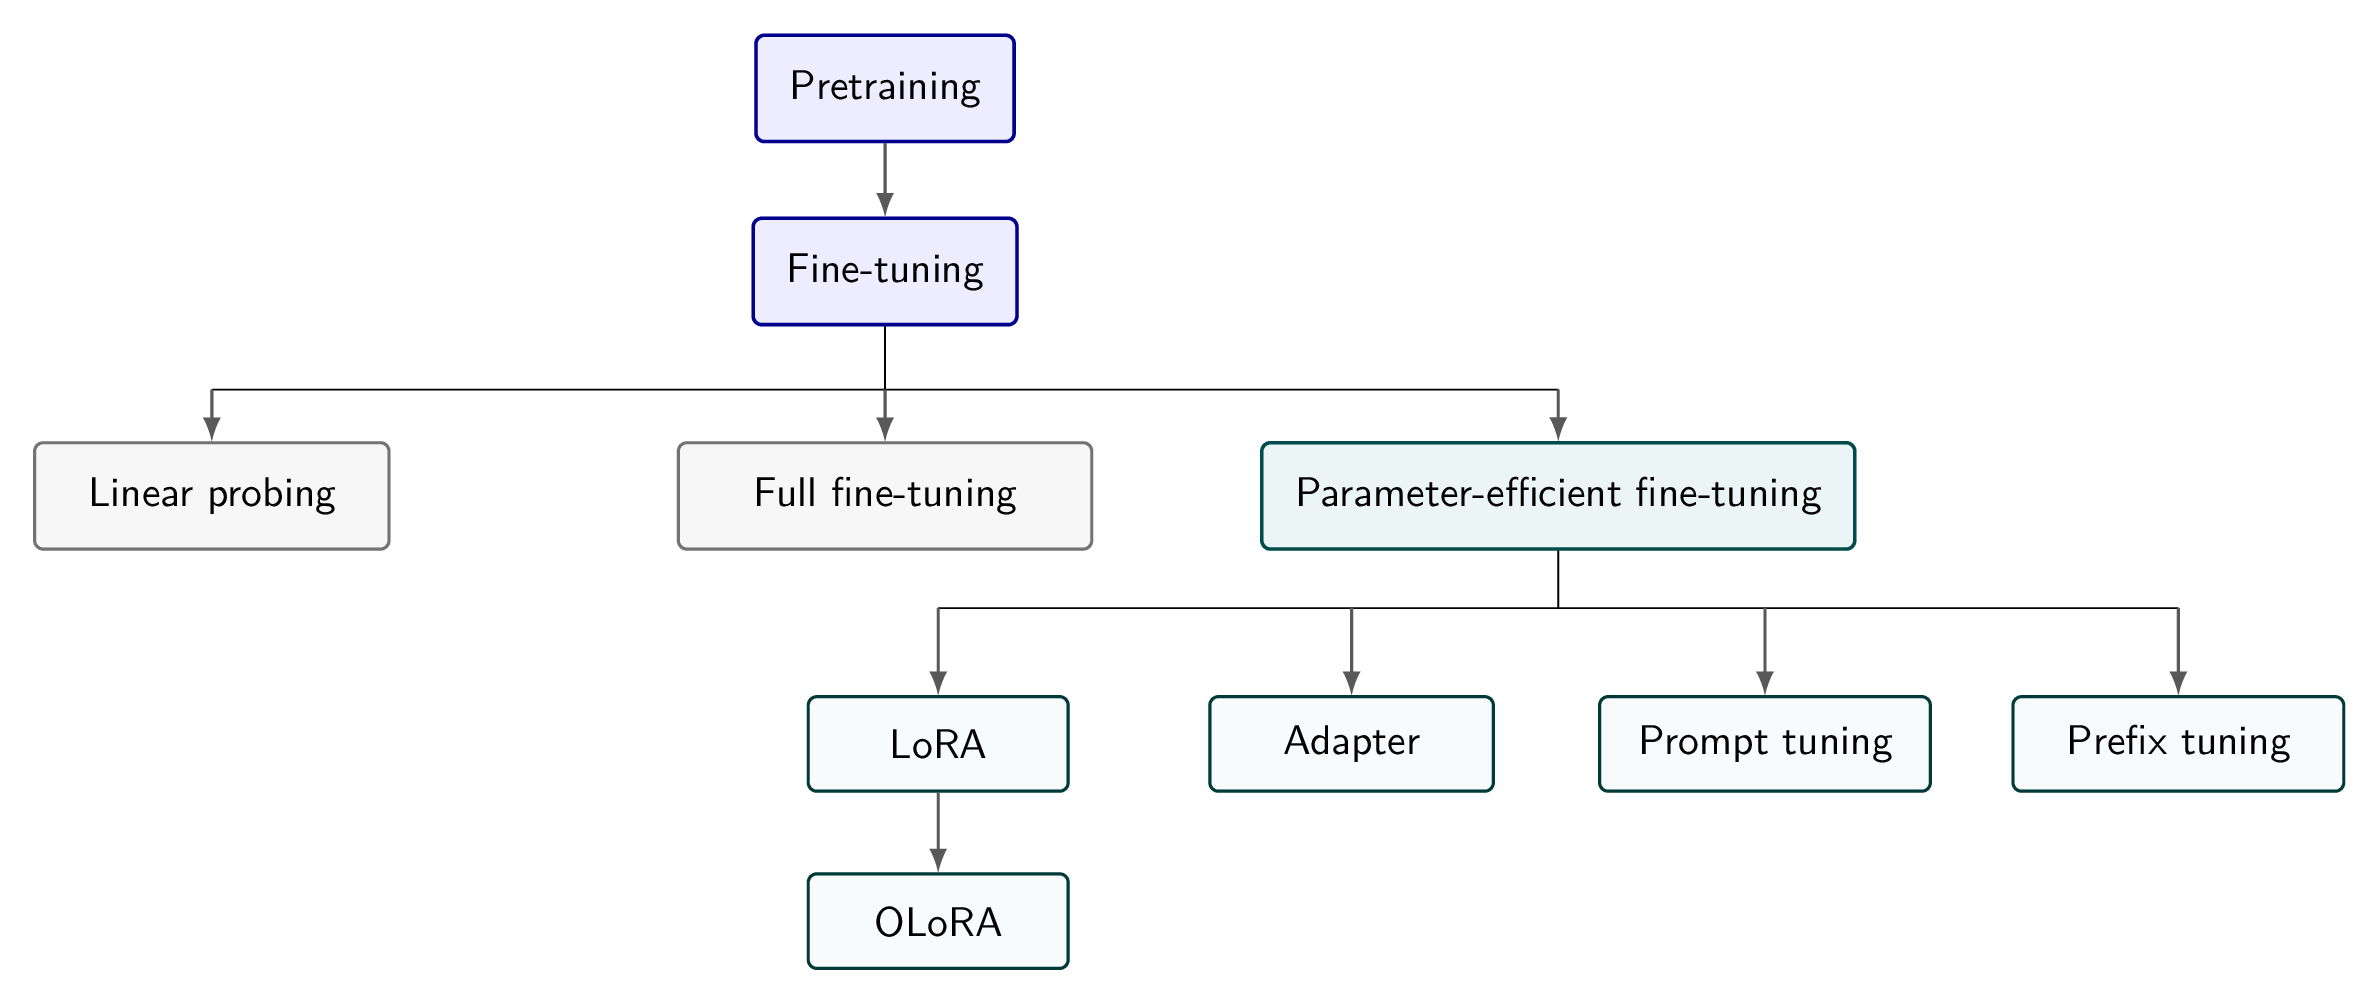
\includegraphics[height=.66\textheight,keepaspectratio]{training_and_finetuning.png}
\par\small Full fine-tuning updates the model. Linear probing trains a head. PEFT trains a small added parameter set, including adapters and LoRA.
\src{Report, Background, Fig. 1; team illustration.}\end{frame}
% Quan: 2 minutes
\begin{frame}{LoRA: a low-rank weight update}
\begin{columns}[T]\column{.48\textwidth}\centering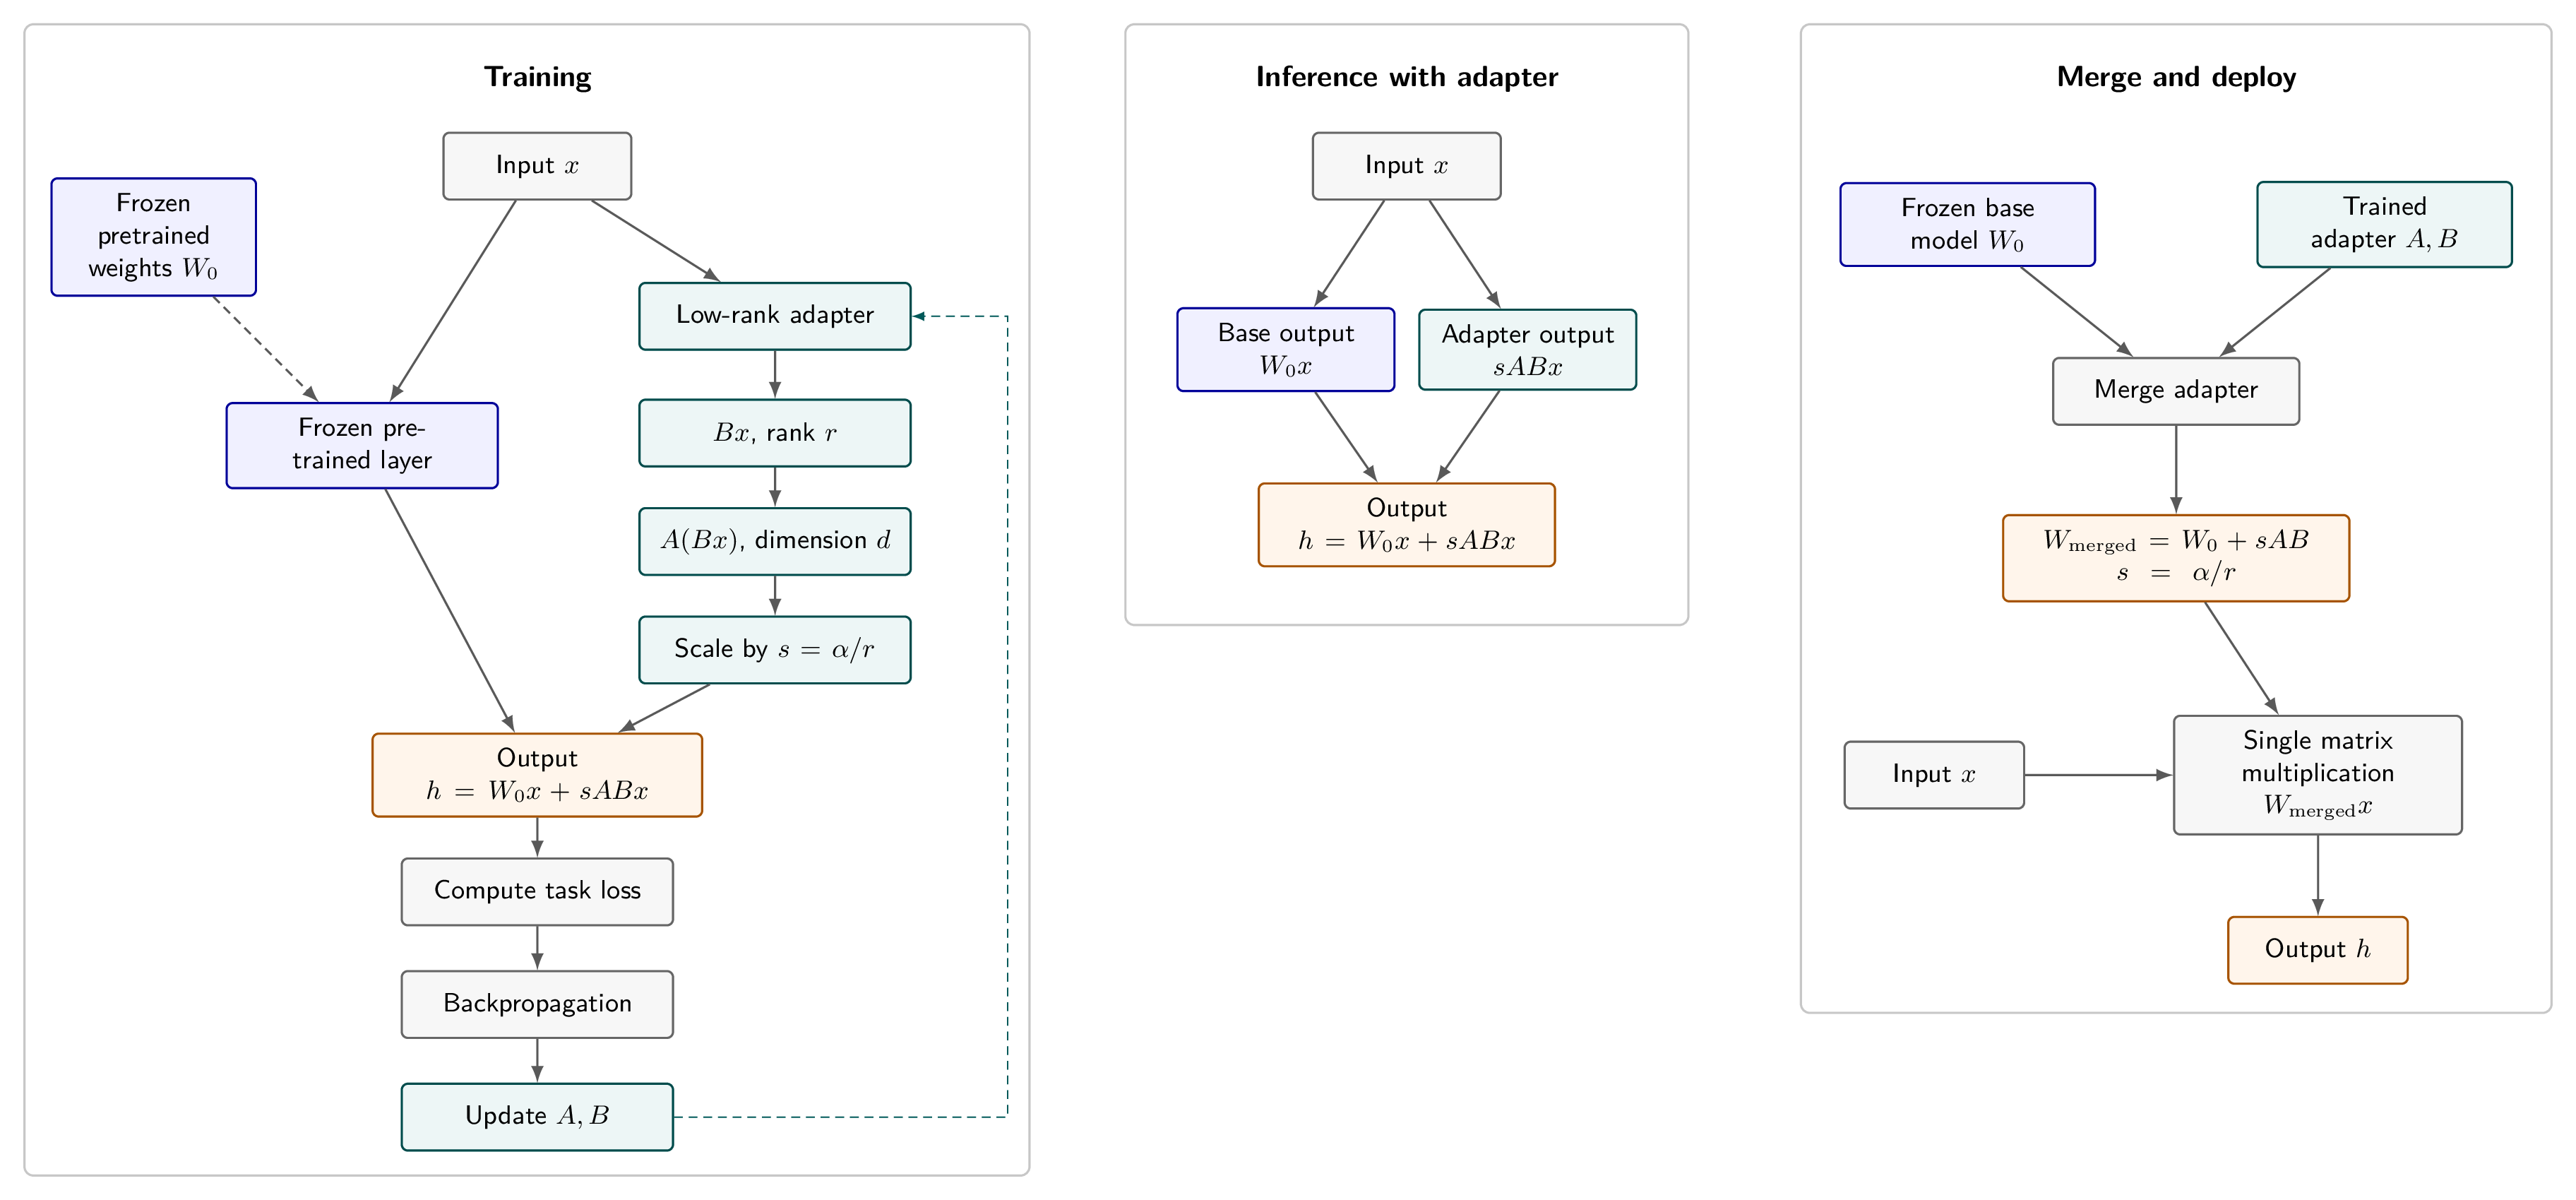
\includegraphics[width=\linewidth]{lora_pipeline.png}
\column{.48\textwidth}\large $W'=W_0+(\alpha/r)AB$\medskip
\begin{itemize}\item $W_0$ stays frozen.\item Train only low-rank $A$ and $B$.\item The pipeline is the team's illustration of Hu et al.'s method.\end{itemize}\end{columns}
\src{Report, Background and Method, Fig. 3; Hu et al. (2022).}\end{frame}
% Lac: 2 minutes
\begin{frame}{LoRA dimensions and scaling}
\centering\Large $h=\left(W_0+\frac{\alpha}{r}AB\right)x$\medskip
\begin{align*}W_0&\in\mathbb R^{d\times k},&A&\in\mathbb R^{d\times r},\\B&\in\mathbb R^{r\times k},&x&\in\mathbb R^k,\quad r\ll\min(d,k).
\end{align*}
\begin{itemize}\item $r$ sets update rank; $\alpha$ scales by $\alpha/r$.\item Only $A,B$ are trained.\item Count assumption: one selected matrix, excluding biases and classifier.\end{itemize}
\src{Report, Method; Hu et al. (2022).}\end{frame}
% Lac: 2 minutes
\begin{frame}{Trainable parameters for a $1024\times1024$ matrix}
\centering\begin{tabular}{lrrr}\toprule
Method&Trainable&Ratio&Reduction\\\midrule
Full fine-tuning&1,048,576&$1\times$&0\%\\
LoRA $r=4$&8,192&$128\times$&99.21875\%\\
LoRA $r=8$&16,384&$64\times$&98.4375\%\\
LoRA $r=16$&32,768&$32\times$&96.875\%\\\bottomrule\end{tabular}
\medskip\par\small $N_{\rm full}=1024^2$; $N_{\rm LoRA}=r(1024+1024)=2048r$.
\par\small GPU memory also holds frozen weights, activations, and temporary tensors.
\src{Report, Method and Worked Example, parameter comparison.}\end{frame}
% Lac: 1 minute
\begin{frame}{LoRA training, inference, and merging}
\centering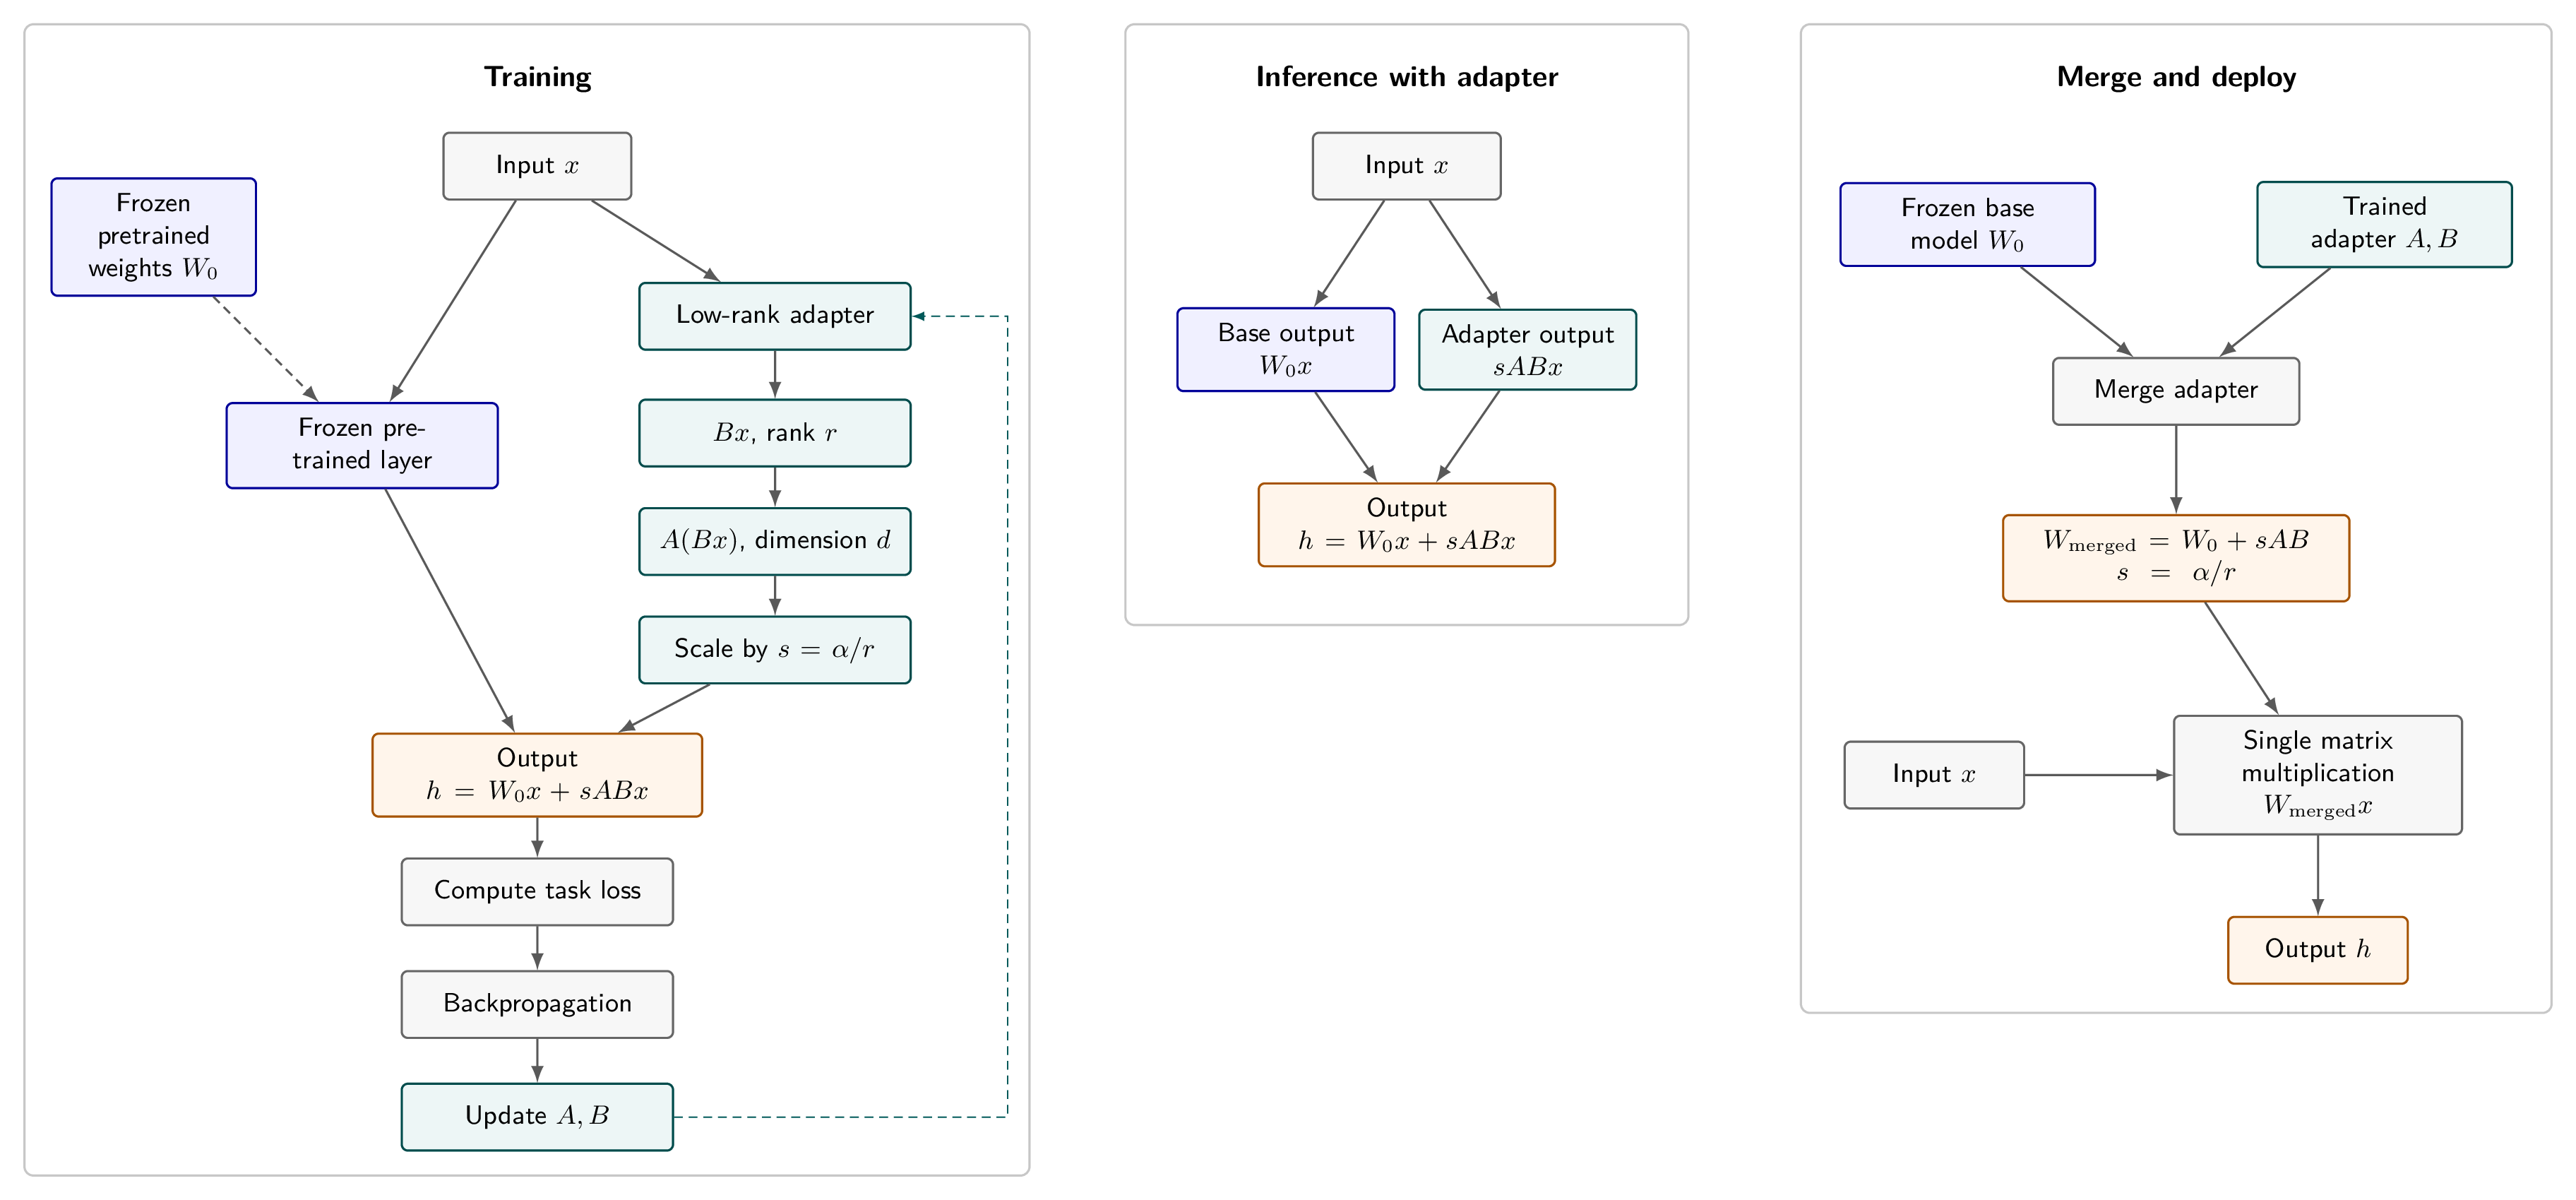
\includegraphics[height=.64\textheight,keepaspectratio]{lora_pipeline.png}
\par\small Training updates $A,B$ while $W_0$ stays frozen. Inference retains the adapter or uses $W_{\rm merged}=W_0+(\alpha/r)AB$.
\src{Report, Method, Fig. 3; Hu et al. (2022).}\end{frame}
% Lac: 1 minute
\begin{frame}{O-LoRA for sequential tasks}
\large $W_t=W_0+\sum_{i=1}^{t}(\alpha/r)A_iB_i$\medskip
\begin{itemize}\item Each task receives its own update; earlier factors remain frozen.\item Add $\lambda\sum_{i<t}\|A_i^\top A_t\|_F^2$ to penalize subspace overlap.\item A finite penalty encourages orthogonality but cannot guarantee zero forgetting.\end{itemize}
\src{Report, Background and Method; Wang et al. (2023).}\end{frame}
% Lac: 2 minutes
\begin{frame}{AG News evaluation: reported run}
\begin{columns}[T]\column{.48\textwidth}\begin{itemize}\item DistilRoBERTa on four-class AG News.\item Planned LoRA: rank 8, $\alpha=16$, query and value adapters plus classifier.\item Official test split: 7,600 examples.\end{itemize}
\column{.48\textwidth}\begin{tabular}{lr}\toprule Metric&Value\\\midrule Accuracy&93.7632\%\\Macro F1&93.7617\%\\Correct&7,126\\Errors&474\\\bottomrule\end{tabular}\end{columns}
\medskip\small Result files do not identify rank or include full fine-tuning results. Metrics characterize the evaluated run only.
\src{Report, Experiment and Results.}\end{frame}
% Tinh: 1.5 minutes
\begin{frame}{Quality and resource trade-offs}
\small\begin{tabular}{p{.22\linewidth}p{.68\linewidth}}\toprule
Measure&Evidence and limit\\\midrule
Quality&93.76\% accuracy and macro F1; no matched full fine-tuning comparison.\\
Memory&Fewer gradients and optimizer states; frozen weights and activations remain. Peak memory was not reported.\\
Training time&No duration was reported.\\
Inference&Merging permits one matrix multiplication; no merged versus unmerged timing was reported.\\\bottomrule\end{tabular}
\src{Report, Results and Discussion; Hu et al. (2022).}\end{frame}
% Tinh: 1.5 minutes
\begin{frame}{Conclusion: when LoRA fits}
\begin{itemize}\item Rank-4 LoRA trains 8,192 instead of 1,048,576 parameters for the worked matrix.\item The evaluated AG News run shows useful performance but cannot establish parity with full fine-tuning.\item LoRA fits when limiting trained parameters matters. Broader changes or inadequate rank may favor another method.\item Verify task quality, GPU memory, training time, and deployment latency. O-LoRA was not evaluated here.\end{itemize}
\src{Report, Conclusion and Results.}\end{frame}
\begin{frame}{References}
\footnotesize\begin{itemize}\item Hu et al. (2022). ``LoRA: Low-Rank Adaptation of Large Language Models.''\item Wang et al. (2023). ``Orthogonal Subspace Learning for Language Model Continual Learning.''\item Zhang et al. (2015). ``Character-level Convolutional Networks for Text Classification.''\item CS420 seminar report, ``LoRA and O-LoRA: Parameter-Efficient Fine-Tuning of Large Models.''\end{itemize}
\medskip Approximately 5 minutes for Q\&A. Each presenter answers at least one question.
\end{frame}
\end{document}
